\begin{figure}[htpb]
    \centering
    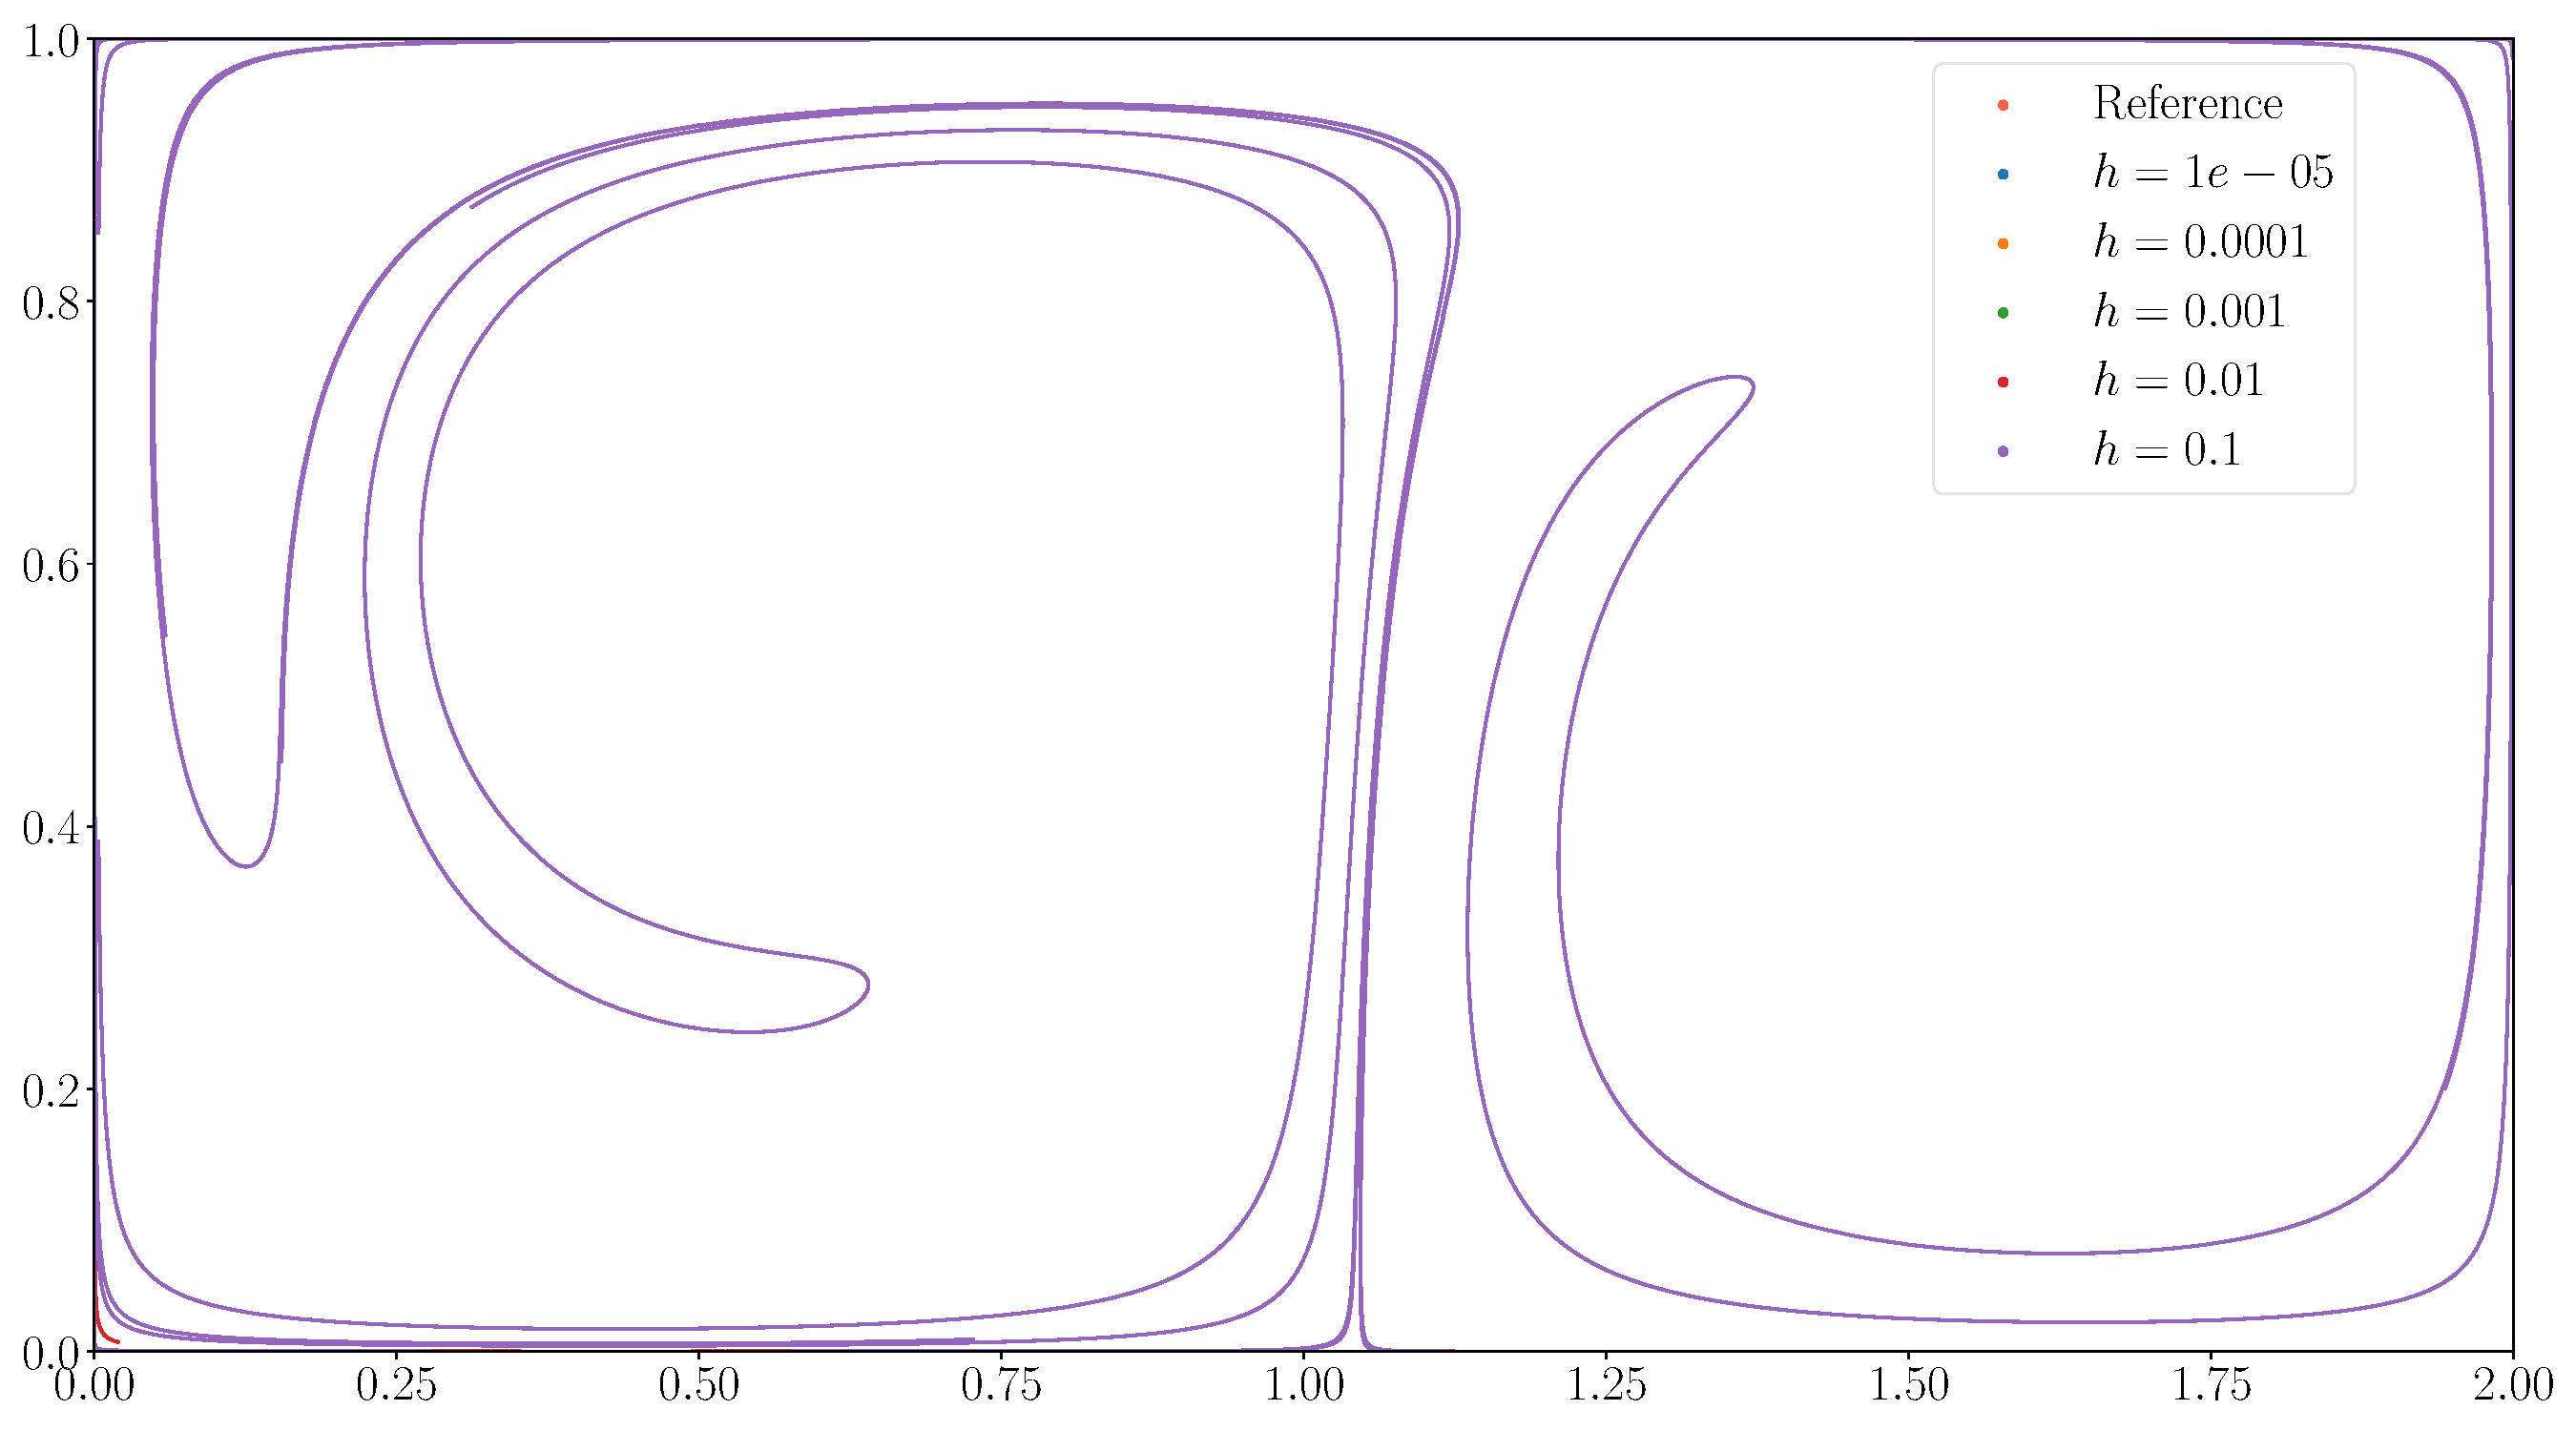
\includegraphics[width=0.8\linewidth]{figures/lcs_figures/rk4.pdf}
    \caption[LCS curves found by means of the classical Runge-Kutta integration scheme]{
        LCS curves found by means of the classical Runge-Kutta integration scheme. The
        reference LCS, as shown by itself in figure~\ref{fig:referencelcs},
        is plotted on the bottom layer. The only visible discrepancy belongs
        to the second largest numerical time step length considered, and is
        located in the lower left corner.}
    \label{fig:lcs_rk4}
\end{figure}
